\documentclass[twoside]{article}
\input{ISC18-english.sty}
%%%%%%%%%%%%%%%%%%%%%%%%%%%%  Make sure to compile twice for proper cross-references. %%%%%%%%%%%%%%%%%%%%%%%
%%%%%%% For proper display of references, compile the document twice. %%%%%%%%%%%%%%%%%%%%% 
%%%%%%%%%%%%%%% If using TeX Live, compile using pdflatex command %%%%%%%%%%%%%%%%%%%%%%%
\begin{document}
\thispagestyle{empty}
%%%%%%%%%%%%%%%%% Article title header  %%%%%%%%%%%%%%%%%%%%
\fancyhead[LE]{Bivariate Quantile Regression Analysis}
%%%%%%%%%%%%%%%%% Article authors header   %%%%%%%%%%%%%%%%%%%%
\fancyhead[RO]{Tourani-Farani, F., Kazemi, I.}
\begin{center}
{
\includegraphics [height=25mm, width=150.3mm] {Images/isc18E}} \\
\vspace*{-1.8cm}
%\begin{center}
%\color{blue} 
%{\hspace{0.1cm}\rule{\textwidth}{1mm}}\\
%\end{center}
\vspace*{4cm}
%%%%%%%%%%%%%%%%% Article title  %%%%%%%%%%%%%%%%%%%%
{\Large \bf Bivariate Quantile Regression Analysis for Longitudinal Cardiovascular Risk Factors}\\
%%%%%%%%%%%%%%%%% Article authors and affiliations %%%%%%%%%%%%%%%%%%%%
{\bf
Fahimeh Tourani-Farani \footnote[1]{{\bf Corresponding Author:} {\tt ft.farani@sci.ui.ac.ir }}, Iraj Kazemi$^2$  \\
$^{1,2}$ Department of Statistics, Faculty of Mathematics \& Statistics, University of Isfahan,Iran
}
\end{center}
\rule{\textwidth}{0.2mm}\\
%%%%%%%%%%%%%%%%% Article abstract  %%%%%%%%%%%%%%%%%%%%
\noindent{\bf Abstract:}\\
Modeling the joint evolution of correlated cardiovascular risk factors across their full distribution remains a statistical challenge, as traditional mean-based longitudinal methods fail to capture extreme-dependent associations and heterogeneous covariate effects. We present a bivariate quantile regression framework for longitudinal data based on the generalized Johnson distribution and the Rosenblatt transformation. The method enables simultaneous modeling of two correlated outcomes at arbitrary quantile levels while preserving interpretability and automatically avoiding quantile crossing. A computationally efficient maximum likelihood estimator is developed with consistency and asymptotic normality guarantees. A comprehensive simulation study demonstrates that the proposed quantile regression model consistently outperforms all competing methods across all evaluation metrics.
 
\noindent{\bf Keywords:} 
 Bivariate analysis, Correlated outcomes, Generalized Johnson distribution, Longitudinal data, Rosenblatt transformation. \\
\noindent{\bf Mathematics Subject Classification (2010):} $\rm 99X99$, $\rm 99X99$, $\rm 99X99$. \\
\hspace{1cm}\rule{\textwidth}{0.2mm}\\
%%%%%%%%%%%%%%
\section{Introduction} \label{sec1}
Longitudinal cardiovascular studies involve repeated measurements of correlated risk factors such as SBP and LDL cholesterol. These outcomes exhibit temporal dependencies and cross-sectional associations \citep{diggle2002analysis,fieuws2004joint}. Understanding covariate effects across the full outcome distribution is clinically critical for identifying vulnerable subpopulations and targeting preventive interventions. %\citep{koenker2005quantile}.\\
Traditional mean-based methods \citep{verbeke1997linear, fitzmaurice2004applied} focus on the conditional mean and fail to capture heterogeneous effects across different quantiles. While univariate quantile regression \citep{koenker1978regression} successfully addresses this limitation for single outcomes, extending this framework to bivariate longitudinal responses remains challenging due to the lack of natural ordering in multivariate spaces and the complexity of modeling joint tail behavior. 
%\citep{ziel2019quantile}.
Several approaches have been proposed to address these challenges. Copula-based methods \citep{nelsen2006introduction, joe2014dependence} provide flexibility in modeling dependence structures but often struggle with high-dimensional settings and quantile-specific inference. Conditional quantile regression methods for longitudinal data \citep{ lai2017quantile, tourani.et.al.2025} have been developed but typically focus on univariate outcomes. To date, a unified framework that simultaneously handles bivariate longitudinal outcomes, arbitrary quantile levels, and heavy-tailed distributions remains lacking \citep{geraci2012quantile, chen2021quantile,sabet2025}.\\
To address these challenges, we introduce a bivariate quantile regression framework integrating the Rosenblatt transformation \citep{rosenblatt1952remarks} with the generalized Johnson distribution \citep{tourani2022transformed}. Our approach offers four key advantages: (1) flexible modeling of skewed and heavy-tailed cardiovascular biomarkers through a rich family of generator functions; (2) automatic quantile non-crossing, preserving stochastic ordering essential for clinical interpretability; (3) quantile-specific dependence structures, allowing correlations between outcomes to vary across risk levels; and (4) interpretable covariate effects across the full distribution. The framework incorporates random effects to account for within-subject correlations in longitudinal settings, with a computationally efficient maximum likelihood estimator providing consistency and asymptotic normality guarantees \citep{laird1982random,jiang2017asymptotic}.\\
The remainder of this paper is organized as follows. Section \ref{sec2} presents the model specification. Section \ref{sec3} describes the estimation procedure. Section \ref{sec4} introduces residual diagnostics. Section \ref{sec5} presents a comprehensive simulation study. Section \ref{sec6} concludes.

%-----------------------
\section{Model Specification} \label{sec2}
Let $\boldsymbol{y}_{t} = (Y_{1t}, Y_{2t})^{\intercal}$ denote a bivariate observation vector at time $t$. The bivariate generalized Johnson (GJS) distribution is characterized by a location vector $\boldsymbol{\gamma}_{t}=(\gamma_{1t},\gamma_{2t})^{\intercal}$, a dispersion matrix $\boldsymbol{\Sigma}_{t}$, a density generator $g(\cdot)$, and transformations $h_1(\cdot), h_2(\cdot)$. The dispersion matrix captures the dependence structure via the Cholesky decomposition $\boldsymbol{\Sigma}_{t} = \boldsymbol{\mathcal{L}}_{t}\boldsymbol{\mathcal{L}}_{t}^{\intercal}$ with $\boldsymbol{\mathcal{L}}_{t} = \begin{pmatrix} \delta_{1t}^{-1} & 0 \\ \rho \delta_{1t}^{-1}\delta_{2t}^{-1} & \delta_{2t}^{-1}\sqrt{1-\rho^2} \end{pmatrix}$, where $\delta_{1t}, \delta_{2t} > 0$ are scale parameters and $|\rho| < 1$ is the correlation coefficient. The spherical representation is $\boldsymbol{\chi}_{t} = \boldsymbol{\mathcal{L}}_{t}^{-1}(h(\boldsymbol{y}_{t}) + \boldsymbol{\mathcal{A}}_{t}\boldsymbol{\gamma}_{t}) \sim S_2(g)$, where $\boldsymbol{\mathcal{A}}_{t} = \text{diag}(\delta_{1t}^{-1}, \delta_{2t}^{-1})$ and $S_2(g)$ denotes a spherical distribution with generator $g$. The resulting density function is
\[
f_{\boldsymbol{y}_{t}}(\boldsymbol{y}) = c_2 |\dot{h}(\boldsymbol{y})| \, |\boldsymbol{\Sigma}_{t}|^{-\frac{1}{2}} g\left((h(\boldsymbol{y}) + \boldsymbol{\mathcal{A}}_{t}\boldsymbol{\gamma}_{t})^{\intercal} \boldsymbol{\Sigma}_{t}^{-1} (h(\boldsymbol{y}) + \boldsymbol{\mathcal{A}}_{t}\boldsymbol{\gamma}_{t})\right),
\]
where $c_2$ is the normalizing constant and $|\dot{h}(\boldsymbol{y})|$ is the determinant of the Jacobian of the transformations.\\
The transformation functions $h_1(\cdot)$ and $h_2(\cdot)$ provide flexibility to accommodate various data types. Common choices include the identity transformation for unbounded outcomes, the logarithmic transformation for positive outcomes, and the logit transformation for bounded outcomes. The generator $g(\cdot)$, required to satisfy $\int_{0}^{\infty} t^{\frac{K}{2}-1} g(u) du < \infty$, determines the tail behavior of the distribution. Special cases include the normal generator $g(u) = \exp(-u/2)/\sqrt{2\pi}$ for light tails and the Student's $t$ generator $g(u) = (1+u/\nu)^{-(2+\nu)/2}$ for heavy tail data sets.\\
For the bivariate GJS distribution, the $p$-th quantile vector $\boldsymbol{Q}^{p}=(Q_{1}^{p},Q_{2}^{p})^{\intercal}$ satisfies
\[
Q_{1}^{p}=h_{1}^{-1}\left(\frac{Q_{1}^{\ast^{p}}-\gamma_{1}}{\delta_{1}}\right), \quad
Q_{2}^{p}=h_{2}^{-1}\left(\frac{Q_{2}^{\ast^{p}}-\gamma_{2.1}}{\delta_{2.1}}\right),
\]
where $Q_{1}^{\ast^{p}}, Q_{2}^{\ast^{p}}$ are spherical generator quantiles, and $\gamma_{2.1} = \frac{\gamma_{2}-\rho \chi_{1}}{\sqrt{1-\rho^{2}}}$, $\delta_{2.1} = \frac{\delta_{2}}{\sqrt{1-\rho^{2}}}$. A key advantage of this construction is the automatic enforcement of quantile non-crossing. Since $Q_{1}^{\ast^{p}}$ and $Q_{2}^{\ast^{p}}$ are strictly monotonic increasing functions of $p$, and $h_{k}^{-1}(\cdot)$ is also strictly increasing, the composite quantile function $Q_{k}^{p}$ preserves monotonicity. Thus, for any $p_{1} < p_{2}$, we have $Q_{k}^{p_{1}} < Q_{k}^{p_{2}}$ for all covariate values, ensuring valid distributional estimates.\\
For longitudinal data, let $\boldsymbol{y}_{it_i}$ denote the response vector for subject $i$ at time $t_i$. For a fixed quantile level $p$, the bivariate quantile regression model is
\begin{equation}
	d_{11}(Q_{it_i,1}^{p}) = \boldsymbol{x}_{1t_i,1}^{\intercal}\boldsymbol{\beta}_1 + b_{i1}, \qquad d_{12}(Q_{it_i,2}^{p})  = \boldsymbol{x}_{1t_i,2}^{\intercal}\boldsymbol{\beta}_2 + b_{i2},
\end{equation}
where $d_{11}(\cdot)$ and $d_{12}(\cdot)$ are strictly monotonic link functions, $\boldsymbol{x}_{1t_i,1}$ and $\boldsymbol{x}_{1t_i,2}$ are covariate vectors (which may include time-varying covariates, time-constant covariates, and their interactions), and $\boldsymbol{\beta}_1$, $\boldsymbol{\beta}_2$ are the corresponding regression coefficient vectors.\\
The dispersion parameters can also be modeled as functions of covariates
\begin{equation}
	d_{21}(\delta_{t,1}) = \boldsymbol{x}_{2t,1}^{\intercal}\boldsymbol{\varsigma}_1, \qquad d_{22}(\delta_{t,2}) = \boldsymbol{x}_{2t,2}^{\intercal}\boldsymbol{\varsigma}_2,
\end{equation}
where $d_{21}(\cdot)$ and $d_{22}(\cdot)$ are monotonic link functions, typically the logarithmic function to guarantee positivity. Subject-specific heterogeneity is captured by random effects $\boldsymbol{b}_i = (b_{i1}, b_{i2})^{\intercal} \sim \mathcal{N}(\boldsymbol{0}, \text{diag}(\sigma_{b1}^2, \sigma_{b2}^2))$, accounting for within-subject correlations.\\
The choice of link functions provides flexibility: $d_{1k}(\cdot)$ can be identity, log, or logit depending on the response type, while $d_{2k}(\cdot)$ typically uses the log link to ensure positivity. The transformations $h_k(\cdot)$ may match the link functions or be chosen independently based on the data characteristics.

\section{Maximum Likelihood Estimation}\label{sec3}

Let $\boldsymbol{y}_{it_i} = (y_{it_i,1}, y_{it_i,2})^{\intercal}$ denote the bivariate response vector for subject $i$ at time $t_i$. Conditional on random effects $\boldsymbol{b}_i = (b_{i1}, b_{i2})^{\intercal}$, responses are independent across time. The likelihood function integrates out the random effects
\begin{equation}
	L(\boldsymbol{\theta}) = \prod_{i=1}^n \int \prod_{t_i=1}^{T_i} f(\boldsymbol{y}_{it_i}|\boldsymbol{b}_i) \, f(\boldsymbol{b}_i) \, d\boldsymbol{b}_i,
\end{equation}
where $\boldsymbol{\theta} = (\boldsymbol{\beta}_1^{\intercal}, \boldsymbol{\beta}_2^{\intercal}, \boldsymbol{\varsigma}_1^{\intercal}, \boldsymbol{\varsigma}_2^{\intercal}, \rho, \sigma_{b1}^2, \sigma_{b2}^2)^{\intercal}$, $f(\boldsymbol{y}_{it_i}|\boldsymbol{b}_i)$ is the conditional GJS density, and $f(\boldsymbol{b}_i)$ is the joint density of independent random effects
\begin{equation}
	f(\boldsymbol{b}_i) = \frac{1}{2\pi \sigma_{b1} \sigma_{b2}} \exp\left(-\frac{b_{i1}^2}{2\sigma_{b1}^2} - \frac{b_{i2}^2}{2\sigma_{b2}^2}\right).
\end{equation}
The integral has no closed form and is approximated using adaptive Gauss-Hermite quadrature (GHQ)
\begin{equation}
	\int \prod_{t_i=1}^{T_i} f(\boldsymbol{y}_{it_i}|\boldsymbol{b}_i) f(\boldsymbol{b}_i) d\boldsymbol{b}_i \approx \sum_{k=1}^{K} \sum_{l=1}^{K} w_k w_l \, \prod_{t_i=1}^{T_i} f(\boldsymbol{y}_{it_i}|b_{k}, b_{l}) \, \frac{1}{\pi} \exp(-b_k^2 - b_l^2),
\end{equation}
where $K$ is the number of quadrature points, $b_k, b_l$ are Gauss-Hermite nodes, and $w_k, w_l$ are weights.\\
The log-likelihood $\ell(\boldsymbol{\theta}) = \log L(\boldsymbol{\theta})$ is maximized using the L-BFGS algorithm with automatic differentiation for exact gradients. Under standard regularity conditions, the maximum likelihood estimator $\widehat{\boldsymbol{\theta}}$ is consistent and asymptotically normal, $\sqrt{n} (\widehat{\boldsymbol{\theta}} - \boldsymbol{\theta}_0) \xrightarrow{d} \mathcal{N}(\boldsymbol{0}, \boldsymbol{I}(\boldsymbol{\theta}_0)^{-1})$, where $\boldsymbol{\theta}_0$ is the true parameter vector and $\boldsymbol{I}(\boldsymbol{\theta}_0)$ is the Fisher information matrix. The asymptotic covariance matrix is estimated by the inverse of the observed Fisher information matrix, $ \left(-\frac{\partial^2 \ell(\widehat{\boldsymbol{\theta}})}{\partial \boldsymbol{\theta} \partial \boldsymbol{\theta}^{\intercal}}\right)^{-1}$. Therefore, the standard errors are obtained from this matrix. The estimation procedure is implemented in \texttt{R} using the \texttt{Stan} probabilistic programming language, which provides efficient automatic differentiation and robust L-BFGS optimization. 
%Convergence is assessed by monitoring the gradient norm and the relative change in the log-likelihood. Optimization is considered converged when the gradient norm falls below $10^{-4}$ and the relative change in log-likelihood between successive iterations is less than $10^{-6}$. For models with random effects, the number of quadrature points $K$ is selected adaptively based on the estimated variance components, with $K = 5$ to $10$ points per random effect providing a favorable balance between computational efficiency and numerical accuracy.
\section{Residual Analysis}\label{sec4}

Model diagnostics are essential for validating the assumptions underlying the proposed framework. We employ quantile residuals, which transform observed responses to approximate standard normal distribution when the model is correctly specified. The quantile residuals are defined as
\begin{equation}
	r_{it_i,1}^{Q} = \Phi^{-1}\left(G_1(r_{it_i,1})\right), \quad
	r_{it_i,2}^{Q} = \Phi^{-1}\left(G_{2.1}(r_{it_i,2})\right),
\end{equation}
where \( G_1(\cdot) \) and \( G_{2.1}(\cdot) \) are the cumulative distribution functions of the spherical generator, and \( \Phi^{-1}(\cdot) \) is the standard normal quantile function. Here, \( r_{it_i,1} \) and \( r_{it_i,2} \) are intermediate residuals defined as
\begin{equation}
	r_{it_i,1} = Q_1^{\ast^{p}} + \widehat{\delta}_{t,1}\left(h_1(y_{it_i,1}) - h_1(\widehat{Q}_{it_i,1}^{p})\right), \quad
	r_{it_i,2} = Q_2^{\ast^{p}} + \widehat{\delta}_{t,2.1}\left(h_2(y_{it_i,2}) - h_2(\widehat{Q}_{it_i,2}^{p})\right),
\end{equation}
where \( \widehat{Q}_{it_i,1}^{p} \) and \( \widehat{Q}_{it_i,2}^{p} \) are the estimated conditional quantiles, \( \widehat{\delta}_{t,1} \) and \( \widehat{\delta}_{t,2.1} \) are the estimated dispersion parameters, and \( Q_1^{\ast^{p}} \), \( Q_2^{\ast^{p}} \) are the quantiles of the spherical generator.\\
Under correct model specification, the quantile residuals \( r_{it_i,1}^{Q} \) and \( r_{it_i,2}^{Q} \) should approximately follow a standard normal distribution. This property follows from the Rosenblatt transformation, which ensures uniformity of \( G_1(r_{it_i,1}) \) and \( G_{2.1}(r_{it_i,2}) \), and the inverse normal transformation that converts uniform distribution to standard normal distribution.

\section{Simulation Study}\label{sec5}

A comprehensive simulation study was conducted to evaluate the proposed bivariate quantile regression model under conditions mimicking real cardiovascular research. The simulation emulated longitudinal trajectories of systolic blood pressure (SBP) and LDL cholesterol with covariates including age, sex, race, education (HS and HS+), and their interactions with age. Synthetic data were generated for 5,000 participants with up to 8 repeated measurements. True parameter values were calibrated from epidemiological literature and preliminary analysis of an undisclosed real dataset. Data were generated using a multivariate Student's $t$-distribution with $\nu = 4$ degrees of freedom to represent heavy-tailed characteristics common in clinical data.\\
The MGJS framework was evaluated using four generators (Normal, Student's $t$, Laplace, Logistic) and compared against linear mixed models (LMM), separate multivariate quantile regression (MQR), and copula-based quantile regression (CQR). Performance metrics included relative bias (\%), root mean square error (RMSE), and rank. Simulations were replicated 500 times. Table~\ref{tab:simulation_results_complete} presents the complete results.
\begin{table*}
	\centering
	\caption{Complete Simulation Results Under Heavy-Tailed Scenario: Bias (\%) and RMSE (Rank shown as SBP/LDL)}
	\label{tab:simulation_results_complete}
	\setlength{\tabcolsep}{2.5pt}
	\renewcommand{\arraystretch}{0.65}
	\footnotesize
	\begin{tabular}{l l c c c c c}
		\hline
		\multirow{2}{*}{Parameter} & \multirow{2}{*}{Method} & \multicolumn{2}{c}{SBP} & \multicolumn{2}{c}{LDL} & \multirow{2}{*}{Rank} \\
		\cline{3-6}
		& & Bias(\%) & RMSE & Bias(\%) & RMSE & \\
		\hline
		\multicolumn{7}{c}{Main Effects} \\
		\hline
		\multirow{6}{*}{Age} & MGJS-Student & 0.09 & 0.00419 & -0.05 & 0.00890 & 1/1 \\
		& MGJS-Laplace & 0.32 & 0.00735 & 0.22 & 0.00965 & 2/2 \\
		& MQR & 0.42 & 0.00680 & 0.23 & 0.01170 & 3/3 \\
		& MGJS-Logistic & 0.40 & 0.00711 & 0.30 & 0.01210 & 4/4 \\
		& MGJS-Normal & 0.55 & 0.00910 & 0.55 & 0.01313 & 5/5 \\
		& LMM & 1.10 & 0.01406 & 1.02 & 0.02030 & 6/6 \\
		\hline
		\multirow{6}{*}{Sex} & MGJS-Student & -0.22 & 0.02644 & -0.01 & 0.22918 & 5/1 \\
		& MGJS-Laplace & -0.16 & 0.02174 & 0.56 & 0.27859 & 4/2 \\
		& MQR & -0.12 & 0.01642 & 0.45 & 0.28029 & 3/3 \\
		& MGJS-Logistic & 0.03 & 0.01148 & 0.59 & 0.30734 & 1/4 \\
		& MGJS-Normal & 0.11 & 0.01487 & 0.64 & 0.34613 & 2/5 \\
		& LMM & 0.38 & 0.04604 & 1.39 & 0.46322 & 6/6 \\
		\hline
		\multirow{6}{*}{Race} & MGJS-Student & -1.36 & 0.02532 & -2.24 & 0.09069 & 1/1 \\
		& MGJS-Laplace & -2.32 & 0.02703 & -2.65 & 0.10703 & 2/3 \\
		& MQR & -2.29 & 0.03463 & -2.52 & 0.10074 & 4/2 \\
		& MGJS-Logistic & -4.09 & 0.04653 & -2.86 & 0.11427 & 5/4 \\
		& MGJS-Normal & -3.25 & 0.03450 & -2.95 & 0.11801 & 3/5 \\
		& LMM & -4.92 & 0.05149 & -3.85 & 0.15403 & 6/6 \\
		\hline
		\multirow{6}{*}{HS} & MGJS-Student & -3.49 & 0.08154 & 8.72 & 0.14439 & 1/1 \\
		& MGJS-Laplace & -4.32 & 0.10333 & 11.81 & 0.17101 & 2/2 \\
		& MQR & -4.24 & 0.10763 & 11.35 & 0.17367 & 3/3 \\
		& MGJS-Logistic & -4.18 & 0.10809 & 12.67 & 0.19470 & 4/4 \\
		& MGJS-Normal & -5.76 & 0.13574 & 12.81 & 0.21200 & 5/5 \\
		& LMM & -7.21 & 0.17647 & 17.55 & 0.27390 & 6/6 \\
		\hline
		\multirow{6}{*}{HS+} & MGJS-Student & -1.04 & 0.09733 & 4.55 & 0.15167 & 1/1 \\
		& MGJS-Laplace & -1.03 & 0.11626 & 5.29 & 0.16796 & 2/2 \\
		& MQR & -1.78 & 0.13107 & 4.68 & 0.17145 & 3/3 \\
		& MGJS-Logistic & -1.67 & 0.15383 & 7.35 & 0.19343 & 4/4 \\
		& MGJS-Normal & -2.79 & 0.17794 & 6.90 & 0.20540 & 5/5 \\
		& LMM & -3.88 & 0.21410 & 10.66 & 0.29212 & 6/6 \\
		\hline
		\multicolumn{7}{c}{Interaction Effects} \\
		\hline
		\multirow{6}{*}{Age $\times$ HS} & MGJS-Student & 0.02 & 0.00347 & -0.61 & 0.00829 & 1/6 \\
		& MGJS-Laplace & 0.20 & 0.00469 & -0.36 & 0.00562 & 4/2 \\
		& MQR & 0.21 & 0.00433 & -0.33 & 0.00544 & 2/1 \\
		& MGJS-Logistic & 0.30 & 0.00442 & -0.44 & 0.00701 & 3/3 \\
		& MGJS-Normal & 0.53 & 0.00644 & -0.25 & 0.00716 & 5/4 \\
		& LMM & 0.89 & 0.01028 & -0.19 & 0.00757 & 6/5 \\
		\hline
		\multirow{6}{*}{Age $\times$ HS+} & MGJS-Student & -0.20 & 0.00473 & 0.00 & 0.00608 & 1/2 \\
		& MGJS-Laplace & 0.15 & 0.00542 & 0.00 & 0.00561 & 3/1 \\
		& MQR & 0.21 & 0.00474 & 0.00 & 0.00754 & 2/3 \\
		& MGJS-Logistic & 0.23 & 0.00655 & 0.00 & 0.00792 & 4/5 \\
		& MGJS-Normal & 0.32 & 0.00756 & 0.00 & 0.00775 & 5/4 \\
		& LMM & 0.85 & 0.01117 & 0.00 & 0.01093 & 6/6 \\
		\hline
		\multirow{6}{*}{Age $\times$ Sex} & MGJS-Student & 0.08 & 0.00089 & 0.00 & 0.00810 & 1/3 \\
		& MGJS-Laplace & 0.005 & 0.00160 & 0.00 & 0.00800 & 3/2 \\
		& MQR & -0.15 & 0.00150 & 0.00 & 0.00729 & 2/1 \\
		& MGJS-Logistic & -0.14 & 0.00267 & 0.00 & 0.00911 & 5/4 \\
		& MGJS-Normal & -0.26 & 0.00267 & 0.00 & 0.00931 & 4/5 \\
		& LMM & -0.83 & 0.00826 & 0.00 & 0.01211 & 6/6 \\
		\hline
		\multirow{6}{*}{Age $\times$ Race} & MGJS-Student & 0.03 & 0.00037 & 2.21 & 0.00242 & 1/1 \\
		& MGJS-Laplace & 0.18 & 0.00178 & 2.45 & 0.00273 & 2/2 \\
		& MQR & 0.28 & 0.00277 & 2.58 & 0.00285 & 3/3 \\
		& MGJS-Logistic & 0.47 & 0.00490 & 2.63 & 0.00293 & 4/4 \\
		& MGJS-Normal & 0.53 & 0.00534 & 2.80 & 0.00318 & 5/5 \\
		& LMM & 1.02 & 0.01038 & 3.30 & 0.00385 & 6/6 \\
		\hline
	\end{tabular}
\end{table*}
The MGJS-Student specification consistently demonstrated superior performance across most parameters, achieving the lowest bias and RMSE. For the primary parameter Age (SBP), MGJS-Student substantially outperformed all competing methods. The linear mixed model showed substantially larger bias and RMSE, highlighting limitations of mean-based methods for extreme quantile inference.\\
The random effects were also estimated within the simulation framework. For both SBP and LDL random effects, MGJS-Student consistently achieved the smallest bias and RMSE, while LMM yielded the poorest performance.\\
The Q-Q plots in Figure~\ref{fig:simulation_diagnostics} align closely with the theoretical quantile lines, confirming adequate model fit.

\begin{figure}[h]
	\captionsetup[subfloat]{labelformat=empty}
	\centering
	\begin{tabular}{cc}
		\subfigure[QQ plot for SBP residuals]{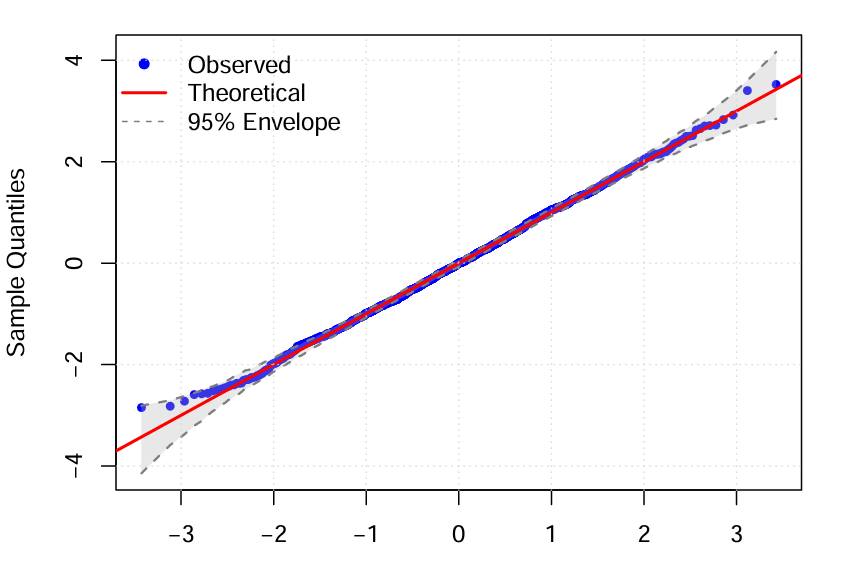
\includegraphics[width=0.45\textwidth]{QQ_Error_ty_1.png}} &
		\subfigure[QQ plot for LDL residuals]{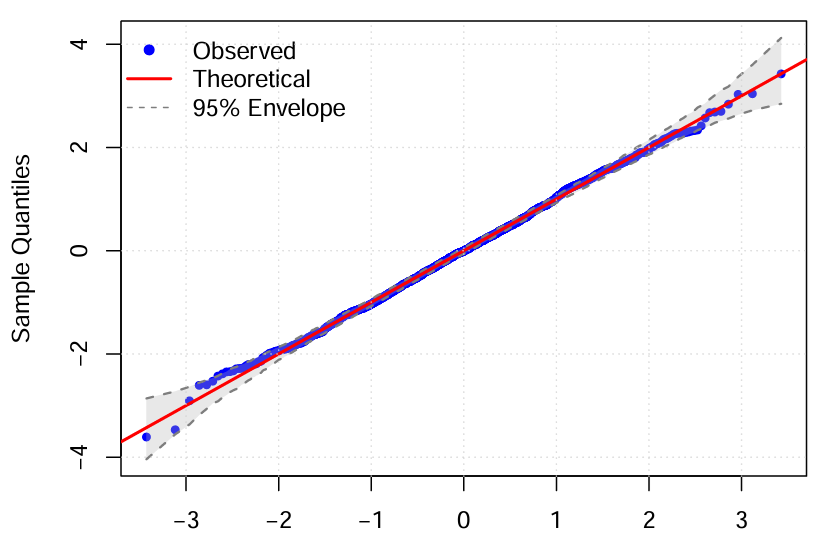
\includegraphics[width=0.45\textwidth]{QQ_Error_ty_2.png}} \\
		%	\subfigure[Histogram of SBP residuals]{\includegraphics[width=0.45\textwidth]{hist_Error_ty_1.png}} &
		%	\subfigure[Histogram of LDL residuals]{\includegraphics[width=0.45\textwidth]{hist_Error_ty_2.png}}
	\end{tabular}
	\vspace{-2mm}
	\caption{QQ plot for (a)  SBP residuals and (b) LDL residuals. %(c) Histogram of SBP residuals; (d) Histogram of LDL residuals.
	}
	\label{fig:simulation_diagnostics}
\end{figure}

The simulation study demonstrates that the MGJS framework, particularly with the Student's $t$ generator, consistently outperforms competing methods across main effects, interactions, and random effects. The clear performance ordering, with MGJS-Student ranked first followed by MGJS-Laplace, MQR, MGJS-Logistic, MGJS-Normal, and LMM last, confirms that heavier-tailed generators provide superior protection against distributional misspecification. Based on these results, MGJS-Student is recommended as the default analytical choice for cardiovascular risk factor research.

\section{Discussion and Conclusion}   \label{sec6}
The proposed bivariate quantile regression framework provides a practical and reliable tool for cardiovascular research. By examining covariate effects across the entire outcome distribution, from normal to high-risk ranges, the method delivers clinically relevant insights that traditional mean-based approaches cannot offer. Simulation results demonstrate that the MGJS-Student framework consistently achieves superior estimation accuracy for extreme quantiles, with automatic quantile non-crossing ensuring logical consistency across risk levels. The current formulation is immediately applicable and offers meaningful advantages over conventional longitudinal methods.
%\section*{Acknowledgments}   
% you wish to include acknowledgments, this section should appear before the references.
%%%%%%%%%%%%%%%%%%%%%%%% References %%%%%%%%%%%%%%%%%%%%%%%%%%%%%
%\newpage
\begin{thebibliography}{0}
\small
%\setlength{\baselineskip}{13pt}
%\setlength{\parskip}{0pt}
%\setlength{\itemsep}{1pt}
	
	\bibitem[Chen et al.(2015)]{lai2017quantile} Chen, X., Sun, J., and Liu, L. (2015). Semiparametric partial linear quantile regression of longitudinal data with time varying coefficients and informative observation times. \textit{Statistica Sinica}, 1437-1458.
	
	\bibitem[Chen et al.(2021)]{chen2021quantile} Chen, X., Li, R., and Wang, Y. (2021). Quantile regression for longitudinal data with random effects. \textit{Journal of Multivariate Analysis}, 184, 104742.
	
	\bibitem[Diggle(2002)]{diggle2002analysis} Diggle, P. (2002). \textit{Analysis of Longitudinal Data} (2nd ed.). Oxford University Press.
	
	\bibitem[Fieuws and Verbeke(2004)]{fieuws2004joint} Fieuws, S., and Verbeke, G. (2004). Joint modelling of multivariate longitudinal profiles: pitfalls of the random-effects approach. \textit{Statistics in medicine}, 23(\textbf{20}), 3093-3104.
	
	\bibitem[Fitzmaurice et al.(2012)]{fitzmaurice2004applied} Fitzmaurice, G. M., Laird, N. M., and Ware, J. H. (2012). \textit{Applied Longitudinal Analysis}. John Wiley and Sons.
	
	\bibitem[Fu and Wang (2012)]{fu2012quantile} Fu, L., and Wang, Y. G. (2012). Quantile regression for longitudinal data with a working correlation model. \textit{Computational Statistics and Data Analysis}, 56(\textbf{8}), 2526-2538.
	
	\bibitem[Geraci and Bottai(2012)]{geraci2012quantile} Geraci, M., and Bottai, M. (2012). Quantile regression for longitudinal data using the asymmetric Laplace distribution. \textit{Biostatistics}, 13(\textbf{1}), 23-37.
	
	\bibitem[Jiang(2017)]{jiang2017asymptotic} Jiang, J. (2017). \textit{Asymptotic Analysis of Mixed effects Models: Theory, Applications, and Open Problems}. CRC Press.
	
	\bibitem[Joe, 2014]{joe2014dependence} Joe, H. (2014). \textit{Dependence Modeling with Copulas}. CRC Press.
	
	\bibitem[Johnson(1949)]{johnson1949systems} Johnson, N. L. (1949). Systems of frequency curves generated by methods of translation. \textit{Biometrika}, 36(\textbf{1/2}), 149-176.
	
	\bibitem[Koenker and Bassett(1978)]{koenker1978regression} Koenker, R., and Bassett, G. (1978). Regression quantiles. \textit{Econometrica: journal of the Econometric Society}, 46(\textbf{1}), 33-50.
	
	
	\bibitem[Laird and Ware(1982)]{laird1982random} Laird, N. M., and Ware, J. H. (1982). Random-effects models for longitudinal data. \textit{Biometrics}, 38(\textbf{4}), 963-974.
	
	\bibitem[Nelsen, 2006]{nelsen2006introduction} Nelsen, R. B. (2006). \textit{An Introduction to Copulas} (2nd ed.). Springer.
	
	\bibitem[Rosenblatt(1952)]{rosenblatt1952remarks} Rosenblatt, M. (1952). Remarks on a multivariate transformation. \textit{The Annals of Mathematical Statistics}, 23(\textbf{3}), 470-472.
	
	\bibitem[Sabetrasekh and Kazemi(2025)]{sabet2025} Sabetrasekh, M., and Kazemi, I. (2025). Longitudinal quantile-based regression models using multivariate asymmetric heavy-tailed distributions and leapfrog HMC algorithm. \textit{Journal of Computational and Applied Mathematics}, 470, 116690.
	
	
	\bibitem[Tourani and Kazemi(2022)]{tourani2022transformed} Tourani-Farani, F., and Kazemi, I. (2022). Transformed mixed-effects modeling of correlated bounded and positive data with a novel multivariate generalized Johnson distribution. \textit{Journal of Multivariate Analysis}, 190, 104954.
	
	\bibitem[Tourani et al.(2025)]{tourani.et.al.2025} Tourani-Farani, F., Aghabazaz, Z., and Kazemi, I. (2025). A class of transformed joint quantile time series models with applications to health studies. \textit{Computational Statistics}, 40(\textbf{3}), 1147-1170.
	
	\bibitem[Verbeke and Molenberghs (1997)]{verbeke1997linear} Verbeke, G., and Molenberghs, G. (1997). \textit{Linear mixed models for longitudinal data}. Springer.
	
	\bibitem[Ziel and Steinert(2019)]{ziel2019quantile} Ziel, F., and Steinert, R. (2019). Quantile regression for the qualifying match of GEFCom2017 probabilistic load forecasting. \textit{International Journal of Forecasting}, 35(\textbf{4}), 1400-1408.
	
	
\end{thebibliography}
 \end{document}

